\chapter{概率图模型概述}
\label{chap:pgm-overview}

一台设备发出报警，维修人员需要判断是否停机检查。设备故障造成的过热和传感器失灵都可能触发报警，因此同一条报警记录可以对应不同的内部状态。判断“有故障”之外，还需要估计故障发生的概率，并结合后续温度读数更新判断。故障概率为$0.02$与$0.45$时，即使模型给出同一个分类结果，停机决策所依据的风险也不同。

设备诊断因而需要一个同时描述故障、温度与报警的分布。\term{概率图模型}（probabilistic graphical model, PGM）将这些随机变量画成节点，用图组织局部依赖，再由局部概率函数组成联合分布。可信的局部依赖假设可以减少需要指定的概率，也为复用计算提供依据。本章沿着设备诊断展开：先说明分布保留了哪些预测信息，再建立图与联合分布的关系，最后区分根据证据查询概率和根据数据确定模型这两类任务。

\section{从单值预测到结构化分布}
\label{sec:pgm-overview-distribution-prediction}

以传感器读数$x$预测设备下一时刻的温度时，模型可以返回$\hat y=f(x)$。这种\term{点预测}（point prediction）用一个数值概括输出，分类任务则用一个类别概括输出。它能直接进入后续决策，但单个结果中包含的信息有限，例如一个温度均值没有说明高温状态出现的概率。

保留这些信息的一种方式是给出\term{预测分布}（predictive distribution）$p(y\mid x)$，描述输入固定后各个输出的可能性。离散输出由每种结果的概率表示，连续输出由概率密度表示，落入某个区间的概率通过积分得到。分布可以同时呈现结果的集中位置、分散程度和多个分离的高概率区域。

图~\ref{fig:pgm-overview-predictive-density}用一个人工设定的温度分布说明这种区别。冷却系统有两种可能工况，预测密度分别集中在$40\,^\circ\mathrm{C}$和$80\,^\circ\mathrm{C}$附近，权重各为一半。两种工况的平均温度是$60\,^\circ\mathrm{C}$，恰好落在两个峰之间的低密度区域。保留完整分布能够同时呈现高温和低温工况；用均值或其中一个峰作点预测，则分别丢失峰的位置或另一种工况的信息。

\begin{figure}[htbp]
  \centering
  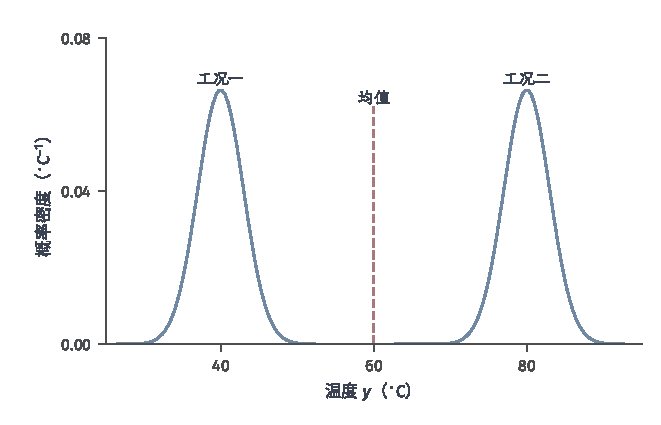
\includegraphics[width=105.412mm]{figures/06-probabilistic-graphical-models/01-representation/matplotlib/pgm-overview-predictive-density/figure.pdf}
  \caption{温度预测中的双峰分布与均值。实线为两个等权高斯密度的混合，每个分量的标准差为$3\,^\circ\mathrm{C}$；虚线标出均值$60\,^\circ\mathrm{C}$。两种工况集中在均值两侧，因而均值这一点预测省略了高概率区域的位置。图中分布为教学设定。}
  \label{fig:pgm-overview-predictive-density}
\end{figure}

预测分布也可以用来产生点预测。设备控制需要一个温度设定值时，可以从分布中选择均值；判断最可能工况时，可以选择概率最大的结果；停机决策则需要把可能的损失一并考虑。分布保留输出的不确定性，具体任务决定怎样将这些信息转化为数值、类别或行动。

当设备包含多个相互影响的部件时，预测还需要联合描述它们的状态。$d$个二值变量共有$2^d$种状态组合，直接指定完整联合表需要$2^d-1$个自由参数。变量数量增加会使数据分散在更多组合中，边缘概率的计算也可能涉及大量状态的汇总。利用局部依赖组织联合分布，正是为了在假设允许的范围内减少参数和计算。

故障与报警之间的联系必须保留，因而把所有变量设为相互独立会损失诊断所需的信息。局部简化可以更有针对性：假设报警只直接依赖过热和传感器失灵，那么给定这两个状态后，故障状态便不再改变报警的局部概率。这种“给定哪些状态后，另一个状态不再提供额外信息”的关系由条件独立表达，并由图结构记录。

\section{图模型上的表示}
\label{sec:pgm-overview-representation}
\label{sec:pgm-overview-basic-concepts}

设备诊断需要同时记录故障、过热、报警和传感器状态。画成图以后，读者不仅要知道哪些状态有关，还要分清哪些量已经观测、哪些量需要推断，以及哪些数值只是模型给定的参数。本节参考PRML第8章的图表示约定，用同一个设备例子说明节点、连线和重复框的含义\scite{bishop2006}。

\paragraph{随机变量与观测状态}
为设备的四种状态分别引入二值随机变量：故障$F$、过热$H$、报警$A$和传感器失灵$S$。每个变量取值$1$表示相应事件发生，取值$0$表示未发生。大写字母表示随机变量，小写$f,h,a,s\in\{0,1\}$表示它们的具体取值；因此$p(f,h,a,s)$是$F=f,H=h,A=a,S=s$同时成立的概率。

圆圈表示随机变量，圈内写变量名称。节点也可以代表一个随机向量，例如把四种状态合为$\bm V=(F,H,A,S)$，图中便可只画一个标有$\bm V$的圆圈。图~\ref{fig:pgm-overview-node-granularity}比较这两种粒度：圆圈的数量并不一定等于标量分量的数量。对于当前尚未取得取值的变量，节点保持空心；已经观测到的变量则给圆圈填色。只有报警记录$A=1$时，$A$画成填色圆圈，$F,H,S$仍为空心。若随后测得过热状态，$H$也改为填色，但模型中的依赖关系不必因此改变。图~\ref{fig:pgm-overview-visual-conventions}对照这两个观测条件，连线保持不变，变化的是节点的填色。

\begin{figure}[!htb]
  \centering
  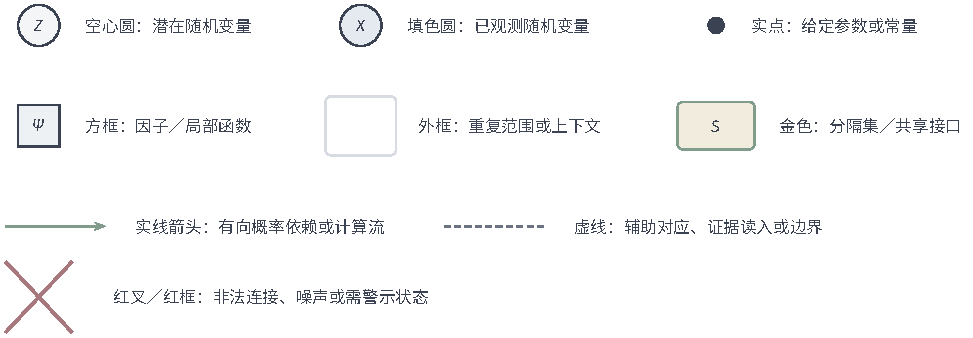
\includegraphics[width=77.646mm]{figures/06-probabilistic-graphical-models/01-representation/tikz/pgm-overview-visual-conventions/figure.pdf}
  \caption{观测信息改变节点填色。(a)仅知报警$A=1$；(b)又测得过热$H=1$。两图使用相同的变量与连线，故障和传感器状态仍未观测；填色表示已有取值，不表示删除随机变量。}
  \label{fig:pgm-overview-visual-conventions}
\end{figure}
\FloatBarrier

\begin{figure}[!htb]
  \centering
  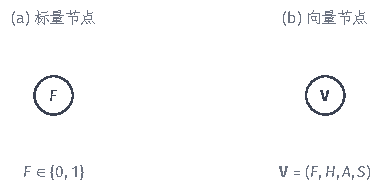
\includegraphics[width=64.703mm]{figures/06-probabilistic-graphical-models/01-representation/tikz/pgm-overview-node-granularity/figure.pdf}
  \caption{圆圈可以表示不同粒度的随机量。(a)一个故障状态$F$；(b)由四种状态组成的随机向量$\bm V$。向量节点并没有把四个分量变成同一个标量，也不表明各分量独立。}
  \label{fig:pgm-overview-node-granularity}
\end{figure}
\FloatBarrier

填色说明这次查询已知什么，不改变变量原本的随机性。空心也不专指模型主动引入的潜变量：尚未观测的故障是当前诊断目标，未来尚未产生的报警也可以是预测目标。对当前记录，模型引入而没有直接观测的内部状态称为潜变量；哪些节点已知、哪些未知，应结合观测条件来读。

只有报警已知而要判断故障时，必须先汇总过热和传感器失灵的可能取值，再按报警概率归一化：
\begin{equation}
  p(f,a)=\sum_{h,s}p(f,h,a,s),
  \qquad
  p(f\mid a)=\frac{p(f,a)}{p(a)},\quad p(a)>0.
  \label{eq:pgm-overview-marginal-conditional}
\end{equation}
这里$\sum_{h,s}$遍历$h,s\in\{0,1\}$的四种组合，$p(a)=\sum_f p(f,a)$；竖线右侧的$a$是已经给定的报警取值。第一式得到故障与报警的边缘概率，第二式使给定报警后故障两种取值的概率之和为$1$。连续变量用相应积分消去，条件分布的基本约定见\BookSectionRef{sec:rv-conditional-distribution}{卷2《数学准备：概率、因果与决策》第1章“随机变量”第1.2.2.2节“条件信息下的分布关系”}。

\paragraph{有向边与局部条件分布}
节点说明模型包含哪些量，连线则组织这些量之间的关系。先不省略任何条件，链式法则给出
\[
  p(f,s,h,a)=p(f)p(s\mid f)p(h\mid f,s)p(a\mid f,s,h).
\]
每一项都保留之前变量的全部取值，因此这种写法并没有减少完整联合表所需的参数。只有进一步指定条件独立关系，才能删去不需要的条件。

条件独立记为$X\perp Y\mid W$，其中$X,Y,W$是随机变量，$x,y,w$是它们各自的取值：给定$W$后，再知道$Y$不会改变$X$的条件分布。对本节的离散变量，在$p(y,w)>0$时可写为$p(x\mid y,w)=p(x\mid w)$；一般条件分布的等式按条件变量的分布几乎处处成立。当前需要的是这些关系怎样简化局部函数，通用独立性约定可参考\BookSectionRef{sec:probability-moments-independence}{卷2《数学准备：概率、因果与决策》第1章“随机变量”第1.2.3节“随机变量的独立关系”}。

设备模型假设故障与传感器失灵独立，过热在给定故障后不再依赖传感器状态，报警在给定过热与传感器状态后不再依赖故障。由此将链式分解中的相应条件删去，得到
\begin{equation}
  p(f,h,a,s)=p(f)p(s)p(h\mid f)p(a\mid h,s).
  \label{eq:pgm-overview-device-joint}
\end{equation}
每个局部条件分布对输出变量归一化，这个乘积就定义了完整联合分布。二值根变量$F,S$各需一个参数；$H$在$F$的两个取值下各需一个参数；$A$在$(H,S)$的四种组合下各需一个参数。总计$8$个自由参数，而完整联合表需要$15$个；减少的参数来自这里采用的独立性假设。

\term{有向图模型}（directed graphical model）用箭头指定局部条件分布使用哪些父变量。进入$A$的两条边$H\to A\leftarrow S$对应$p(a\mid h,s)$；$F\to H$对应$p(h\mid f)$；没有进入$F,S$的边，所以它们分别使用$p(f),p(s)$。图~\ref{fig:pgm-overview-device-graph}画出这一对应。箭头先表示概率分解中的条件关系，因果解释需要额外假设；它也不表示算法必须按箭头方向传递查询信息。第~\ref{chap:pgm-directed}章进一步说明有向分解与条件独立的对应。



\begin{figure}[!htb]
  \centering
  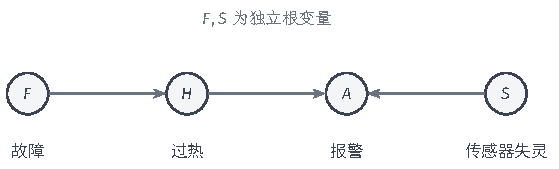
\includegraphics[width=94.590mm]{figures/06-probabilistic-graphical-models/01-representation/tikz/pgm-overview-device-graph/figure.pdf}
  \caption{设备诊断的有向表示。节点表示随机变量，进入节点的箭头指定其局部条件分布所依赖的变量，例如$H\to A\leftarrow S$对应$p(a\mid h,s)$。这里的箭头记录概率分解，因果解释需要另行给出假设。}
  \label{fig:pgm-overview-device-graph}
\end{figure}

\FloatBarrier

\paragraph{固定量与参数节点}
图规定局部函数可以使用哪些变量，函数中的数值还需另外指定。例如，令$\bm\theta_A$收集四种$(h,s)$组合下的报警概率$p(A=1\mid H=h,S=s)$。查询故障时，若这张概率表已经给定，$\bm\theta_A$就是固定量，可以画成小实点，再连到使用它的报警节点。图~\ref{fig:pgm-overview-parameter-roles}(a)只保留报警与其固定参数，显示小实点的作用。

填色大圆圈与小实点承担不同职责：前者是模型中的随机变量，只是本次已经取得取值；后者在当前概率模型中作为给定量使用，不需要对它建立概率分布。固定输入也可以用小实点表示，例如回归中给定的输入位置。参数是否画成实点取决于建模方式，而不是它被称为“参数”：若要为参数本身指定先验并推断其分布，就应将它画成随机变量圆圈。图~\ref{fig:pgm-overview-parameter-roles}(b)用$\bm\Theta_A$表示随机参数，$\bm\theta_A$仍表示它的一种取值。具体参数学习方式由第~\ref{chap:pgm-parameter-learning}章介绍。

\begin{figure}[!htb]
  \centering
  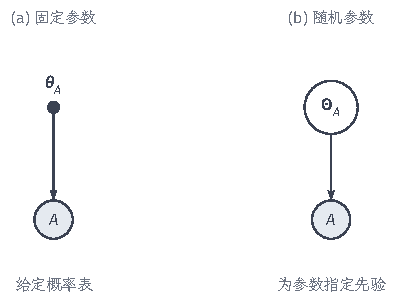
\includegraphics[width=67.165mm]{figures/06-probabilistic-graphical-models/01-representation/tikz/pgm-overview-parameter-roles/figure.pdf}
  \caption{同一参数的两种建模方式。左图将报警表作为固定量，右图为参数$\bm\Theta_A$指定先验，使用随机变量圆圈。两图都观测报警$A$，均省略$H,S$及其入$A$的箭头；实点与填色圆圈不是同一类对象。}
  \label{fig:pgm-overview-parameter-roles}
\end{figure}
\FloatBarrier

同一张图配上不同的局部概率表，会给出不同的诊断结果。图结构组织允许的依赖，参数与局部函数确定具体概率；为保持图简洁，已经在正文说明的固定参数可以不全部画出。

\paragraph{重复框与共享参数}
多台设备采用相同诊断模型时，每条记录都有自己的$F_i,H_i,A_i,S_i$。若逐条画出，节点和连接会大量重复。\term{板表示法}（plate notation）用一个框圈住代表性节点及其连接，再用$N$标出重复次数；下标$i=1,\ldots,N$说明框内变量按记录复制。图~\ref{fig:pgm-overview-plate-expansion}取$N=3$对照展开图和板框图，只保留过热、传感器失灵与报警这三个节点；省略的故障节点也随记录复制。框外的$\bm\theta_A$不复制，而是由每套报警节点共同使用。

\begin{figure*}[!htb]
  \centering
  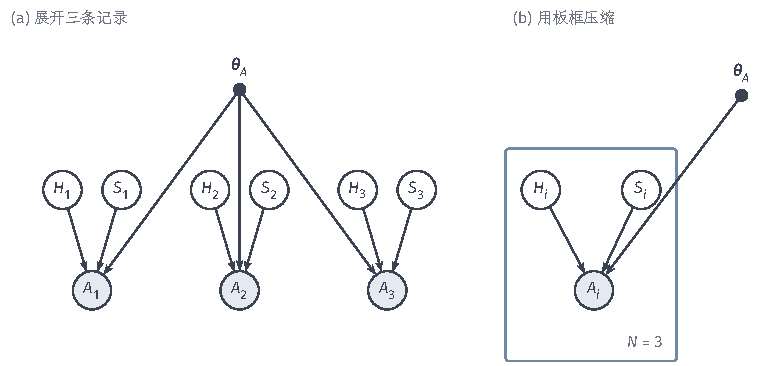
\includegraphics[width=128.926mm]{figures/06-probabilistic-graphical-models/01-representation/tikz/pgm-overview-plate-expansion/figure.pdf}
  \caption{重复框与展开图，取三条记录作图示。左图有三个过热、三个传感器和三个报警变量，三组报警共用一个固定参数；右图用$N=3$的板框压缩这些副本。两图均省略故障变量及相关箭头，框外参数不随记录复制。}
  \label{fig:pgm-overview-plate-expansion}
\end{figure*}
\FloatBarrier

若各记录在给定整组固定参数$\bm\theta$后相互独立，用$p_{\bm\theta}$表示采用这组参数的分布，则重复图对应的联合概率为
\begin{equation}
  p_{\bm\theta}(f_{1:N},h_{1:N},a_{1:N},s_{1:N})
    =\prod_{i=1}^{N}p_{\bm\theta}(f_i,h_i,a_i,s_i).
  \label{eq:pgm-overview-plate-product}
\end{equation}
$\bm\theta$包含四类局部概率表的全部参数，$f_{1:N}$表示$f_1,\ldots,f_N$，其余下标同理。每条记录使用相同的函数形式和参数，但保留自己的状态取值。框本身只表示重复，不单独保证记录独立；若副本之间另有连接，或共享的随机量被边缘化，就要按展开后的依赖关系计算联合分布。

\paragraph{无向边与因子节点}
若重点是邻近部件状态之间的对称相互作用，可以使用\term{无向图模型}（undirected graphical model）。无向边没有箭头，不指定哪个端点作为另一个端点的条件；局部关系由非负势函数评价配置的相对权重。令$\bm x$为全部变量的取值，$c$为局部作用范围的索引，$\bm x_c$为该范围内的取值子向量，则
\[
  p(\bm x)=\frac{1}{Z}\prod_c\psi_c(\bm x_c),
  \qquad
  Z=\sum_{\bm x}\prod_c\psi_c(\bm x_c).
\]
$\psi_c\geq0$是局部势，$Z$是对全部候选配置求和的归一化常数。离散情形下$p(\bm x)$表示联合概率，连续情形下表示密度；连续状态改用积分，且须满足$0<Z<\infty$。无向边表示模型允许的局部相互作用，不等同于两个变量的边缘相关系数。其条件独立语义在第~\ref{chap:pgm-undirected}章展开。

局部函数也可以单独画出来。\term{因子图}（factor graph）用圆圈表示变量、方框表示因子，连接线说明函数用到了哪些变量。例如，令$g_A(a,h,s)=p(a\mid h,s)$，相应的$g_A$方框连接$A,H,S$。这三条无箭头连线表示函数的三个自变量，并不是新增三条随机变量之间的无向边；$g_A$也不需要被观测或赋予一个随机取值。图~\ref{fig:pgm-overview-edge-types}进一步对照无向变量边和一个三变量因子的连线：左图直接连接变量，右图把局部函数单独画出。

\begin{figure}[!htb]
  \centering
  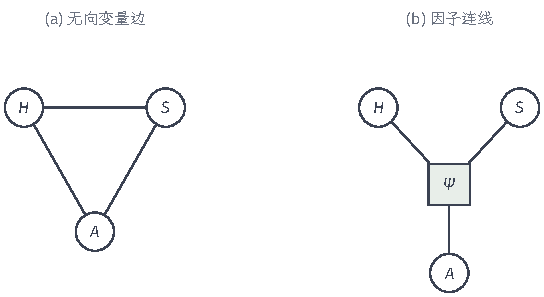
\includegraphics[width=92.135mm]{figures/06-probabilistic-graphical-models/01-representation/tikz/pgm-overview-edge-types/figure.pdf}
  \caption{无向边与变量—因子连线的对象不同。左图允许$H,S,A$组成一个三变量局部作用范围，右图将该范围的势函数$\psi(h,s,a)$显式画成方框。右图的每条线连接一个变量和一个函数，不能读成新增的变量之间连线；两图均不标注观测证据。}
  \label{fig:pgm-overview-edge-types}
\end{figure}
\FloatBarrier

有向模型的条件概率乘积和无向模型的势函数乘积都能画成因子图。圆圈与方框的区别使每个乘积项的作用范围显式可见；原来的父子方向则要由局部函数的含义说明。因此，因子图提供的是乘积分解的计算表示，第~\ref{chap:pgm-representations}章将比较不同表示保留的信息。

算法图中的消息箭头、辅助虚线、分隔集色框和警示颜色由相应图注说明；它们不属于上述概率图节点与边的通用语义，不能只凭颜色或线型判断模型含义。

\FloatBarrier

\section{图模型上的推断与学习}
\label{sec:pgm-overview-inference-learning}

报警记录提出的查询是$p(F=1\mid A=1)$。在图结构和局部概率已知时，根据证据计算这种查询称为\term{概率推断}（probabilistic inference）。过热$H$和传感器状态$S$仍然未知，所以推断要把它们可能处于的每一种状态都纳入后验计算。

为观察计算量如何变化，将诊断范围扩展到更多部件，并设共有$30$个未观测的二值状态，包括$H,S$以及新增的部件或运行状态。将它们统一记为$\bm{Z}=(Z_1,\ldots,Z_{30})$，仍以报警$A=1$为证据、故障$F$为查询目标。后验的分子汇总故障发生时的未知配置，分母汇总故障两种取值下的配置：
\begin{equation}
  p(F=1\mid A=1)
  =
  \frac{
    \displaystyle\sum_{\bm{z}\in\{0,1\}^{30}}
    p(F=1,A=1,\bm{z})
  }{
    \displaystyle\sum_{f\in\{0,1\}}
    \sum_{\bm{z}\in\{0,1\}^{30}}
    p(f,A=1,\bm{z})
  }.
  \label{eq:pgm-overview-expanded-diagnosis}
\end{equation}
直接展开该式时，分子包含$2^{30}$个未观测状态配置，约为$10.7$亿项；分母同时遍历故障的两个取值，包含$2^{31}$个完整配置项，约为$21.5$亿项。这是对状态组合的计数，所需模型参数仍由局部函数决定。

对于一个完整配置$p(f,A=1,\bm{z})$，局部分解允许逐项查表或计算，再将结果相乘。后验却要汇总许多这样的配置，因此主要开销可能来自求和，而非单次乘积评价。若不同配置共享某些局部计算，图结构便可能帮助复用这些结果；复用范围和中间结果大小取决于变量之间的连接方式。

\term{精确推断}（exact inference）重组概率运算，在给定模型下求出原查询的准确答案，其时间和空间开销受问题规模及中间结果大小影响。预算不足以容纳这些中间计算时，可以采用\term{近似推断}（approximate inference），在可承受的时间或空间内估计查询，并分析所引入的误差。第~\ref{chap:pgm-elimination}章至第~\ref{chap:pgm-sampling}章分别讨论这些计算方法及其适用结构。

设备运行记录可以用来确定局部概率的数值。例如，在故障和过热状态均被记录时，故障设备中过热的比例可以用于估计$p(H=1\mid F=1)$。在图结构和局部函数形式给定的前提下估计这些数值，称为\term{参数学习}（parameter learning）。稀有状态只有少量样本时，估计受随机波动影响较大；存在缺失或潜变量时，还需要处理无法直接取得的状态计数。

若设备内部哪些状态应当直接相连也未知，就需要根据数据和领域约束选择图，这称为\term{结构学习}（structure learning）。增加连接可以描述更多依赖，通常也会扩大局部函数并增加估计和推断的开销；减少连接则需要确认相应独立性假设是否适合数据。学习所得的有向结构首先描述概率关系，因果解释仍取决于额外假设和证据。

这两类学习任务确定模型，而推断利用给定模型计算未知状态的概率。含有未观测变量的数据将二者联系起来：参数更新所需的统计量可能依赖潜在状态，于是先用当前模型计算这些状态的后验，再据此更新参数。第~\ref{chap:pgm-parameter-learning}和第~\ref{chap:pgm-structure-learning}章将分别展开参数估计与结构选择。

\section{概率图模型的历史}
\label{sec:pgm-overview-history}

局部相互作用如何组成整体分布，观测如何改变未知状态的概率，未知参数又如何从数据中估计，这些问题推动了概率图模型的发展。图~\ref{fig:pgm-overview-history}与图~\ref{fig:pgm-overview-history-recent}按时间展示代表工作，以下结合各自处理的计算与建模问题说明它们的联系。

\begin{figure*}[p]
\centering
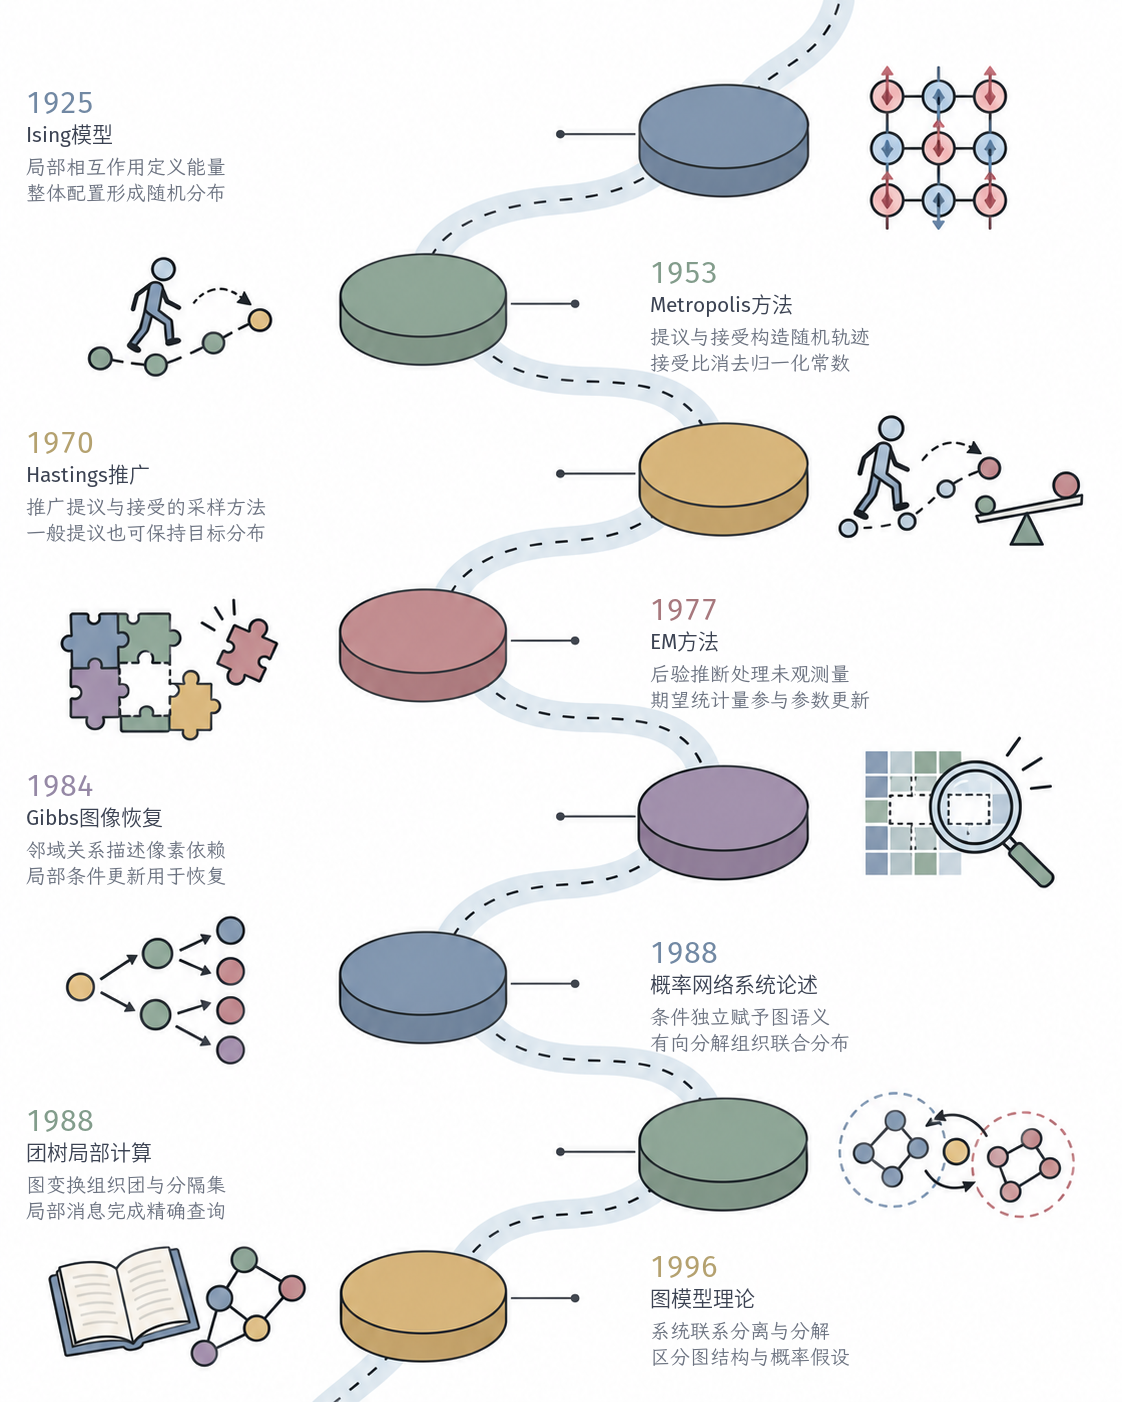
\includegraphics[width=157.406mm,height=.88\textheight,keepaspectratio]{figures/06-probabilistic-graphical-models/04-models/generated/pgm-models-history/figure.png}
\caption{概率图模型发展的代表工作（1925—1996）。沿虚线路线从上向下阅读：局部相互作用组织联合分布，随机更新估计难以直接计算的查询，潜变量学习处理缺失状态，图语义与消息计算联系独立性和推断。1988年Pearl的节点对应系统论述，而非概率网络的首次提出；节点间距不按时间比例绘制。}
  \label{fig:pgm-overview-history}
\end{figure*}
\begin{figure*}[p]
\centering
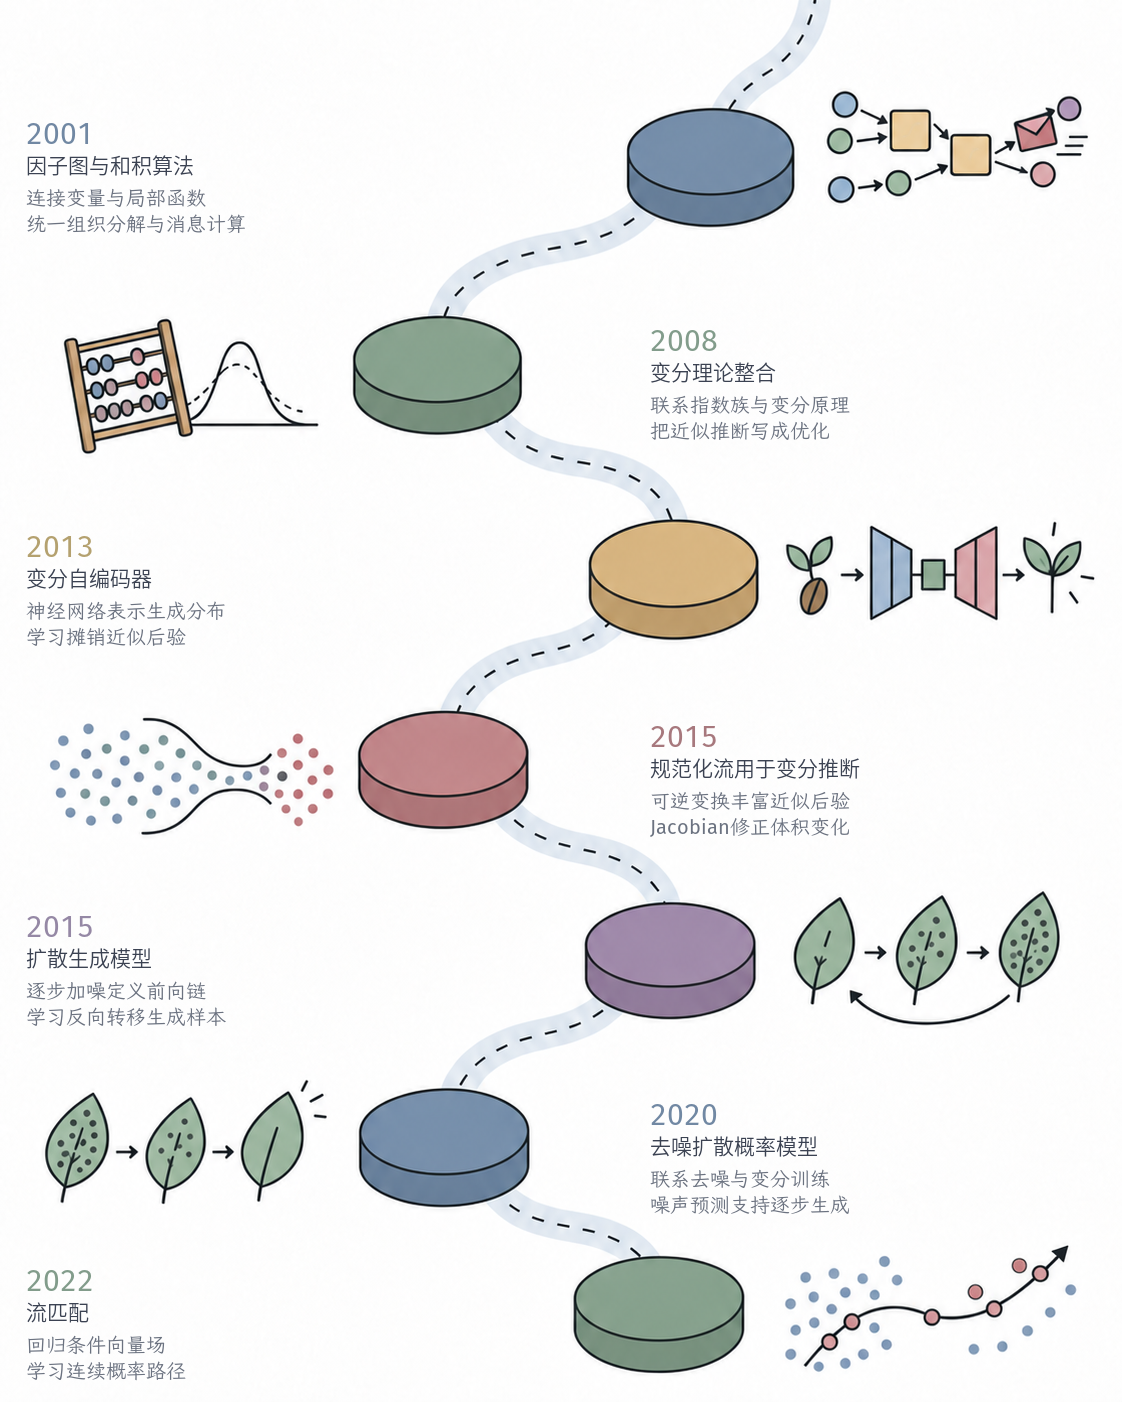
\includegraphics[width=157.406mm,height=.88\textheight,keepaspectratio]{figures/06-probabilistic-graphical-models/01-representation/generated/pgm-models-history-recent/figure.png}
\caption{概率图模型发展的代表工作（2001—2022），承接图~\ref{fig:pgm-overview-history}。因子图组织局部函数与消息，变分理论统一近似推断的优化表述，神经参数化进一步扩展后验近似和生成路径。2008年对应理论整合工作，2015年的规范化流对应流式变分推断；年份采用代表文献的首次公开或发表时间，不表示各类方法的统一起点。}
  \label{fig:pgm-overview-history-recent}
\end{figure*}

\subsection{从局部随机规律到图结构语义}

1925年的Ising模型以相邻自旋的相互作用描述整体配置，是无向局部随机模型的早期代表。每个局部项只涉及少量自旋，而归一化常数与边缘概率仍涉及整体状态的汇总。另一类问题来自数据中的未观测变量：1977年的EM方法利用当前模型推断相关统计量，再让这些统计量参与参数更新\scite{pgm-overview-ising1925,pgm-overview-dempster1977}。

归一化常数难以直接求出时，状态更新提供了另一条计算路线。1953年的Metropolis方法及1970年的Hastings推广通过提议候选状态与决定是否接受，构造随机轨迹；接受比中共同的未知归一化常数可以消去。由轨迹估计查询的效率还取决于链能否充分探索不同状态。1984年的Geman与Geman将局部相互作用定义的Gibbs分布与随机更新用于图像恢复，使局部依赖同时参与分布描述和状态计算\scite{pgm-history-metropolis1953,pgm-history-hastings1970,pgm-history-geman1984}。

1988年Pearl对概率网络的系统论述将条件独立与有向分解联系起来。同年Lauritzen与Spiegelhalter通过图变换组织局部消息，形成一般网络上的精确计算方法；1996年Lauritzen进一步系统整理图模型理论。这些工作分别为概率分解的合法性和查询的计算方式提供依据，而具体查询的开销仍由图结构决定\scite{pgm-pearl1988,pgm-overview-lauritzen1988,pgm-lauritzen1996}。

% 保留小节标题与首段，避免两页历史插画夹断近似推断的说明。
\Needspace{10\baselineskip}
\subsection{学习、近似推断与神经参数化}

大规模模型中的后验计算促使近似推断进一步发展。变分方法在可计算的分布族中优化后验近似，误差与所选分布族及优化结果有关；采样方法通过随机轨迹估计查询，有限时间内的误差与链的探索和混合行为有关。Wainwright与Jordan在2008年的综述系统联系了指数族、变分原理和图上计算\scite{pgm-wainwright2008}。

2013年以来，神经网络进入了分布及推断的参数化：VAE同时表示生成分布与近似后验，规范化流以可逆变换构造密度，扩散模型学习逆转人为加入的噪声过程。各路线提供更灵活的局部函数，同时采用不同的似然评价、后验近似和样本生成方法，因此具有不同的计算代价\scite{kingma2013,pgm-overview-rezende2015,pgm-overview-sohl2015}。

\subsection{当前研究方向}

复杂观测数据需要灵活的分布，同时也需要可承受的后验计算。一类研究设计便于计算的分解，或学习由观测直接给出后验近似的摊销方法，并评价近似误差与校准。另一类研究面向高维条件生成，考察潜变量、可逆变换、扩散和连续流分别怎样表示条件分布、怎样生成样本。流匹配通过拟合条件向量场学习连续生成路径，是其中的代表方法\scite{lipman2023flowmatching}。

对于不完整、多模态或受领域约束的数据，还需检查模型假设的依赖能否由观测识别。除生成样本的质量外，也应分别评价分布表示的准确程度、参数学习的收敛性和预测概率的可靠程度。

\section{本章小结}
\label{sec:pgm-overview-summary}

设备诊断既要判断状态，也要估计状态的概率。联合分布保留了状态间的依赖，却增加了参数和计算量。概率图模型用条件独立假设组织局部函数，并据此简化分布表示与查询计算。

有向图通过局部条件分布分解联合概率，无向图通过势函数乘积与全局归一化表示联合概率，因子图则呈现选定的局部乘积。推断在给定模型下计算概率查询，开销取决于图结构；参数学习与结构学习根据数据确定模型，潜变量使学习与推断相互联系。

下一章从有向图出发，说明条件独立与联合分解的关系。

\paragraph{扩展阅读}
Bishop的PRML第8章解释概率分解与图表示的对应；Koller与Friedman的教材进一步展开表示、推断和学习及其计算结构\scite{bishop2006,pgm-koller2009}。
